\setchapterpreamble[u]{\margintoc}
\chapter{Շատ փոփոխականի ֆունկցիա}
\labch{multi_var}

\emergencystretch 2em

\section{$f(x, y)$-ի գրաֆիկը}\label{3d_graph}

Համարենք, որ ծիրանի գործն ավարտեցինք, և վերադառնանք մեկից ավելի ապրանքների դեպքին, երբ ունենք ֆունկցիա՝ կախված մի քանի փոփոխականներից՝
\[
f(x,y) = x^{2}+y^{2}+e^{y-x}
\]

Ինչպե՞ս այս դեպքի համար ևս մշակենք գործիքներ, որոնցով կկարողա\-նանք գտնել $x$-ի ու $y$-ի այն արժեքները, որոնցում ֆունկցիայի արժեքն ամենամեծը/ամենափոքրն է։ 

Սկսենք ֆունկցիան պատկերելուց։ Նախ՝ փոփոխականը ոչ թե մեկն է, այլ երկուսը․ յուրաքանչյուր $(x, y)$ զույգի համապատասխանում է մեկ արժեք։ Հետևաբար ֆունկցիան պատկերելու համար անհրաժեշտ է
\begin{itemize}
    \item $xy$-հարթությունը՝ արգումենտների համար\marginnote[*+1]{կանվանենք՝ $z$-երի առանցք}
    \item ավելացրած մի նոր առանցք՝ արժեքները նշելու համար
\end{itemize}

\begin{figure}[h]
    \centering
    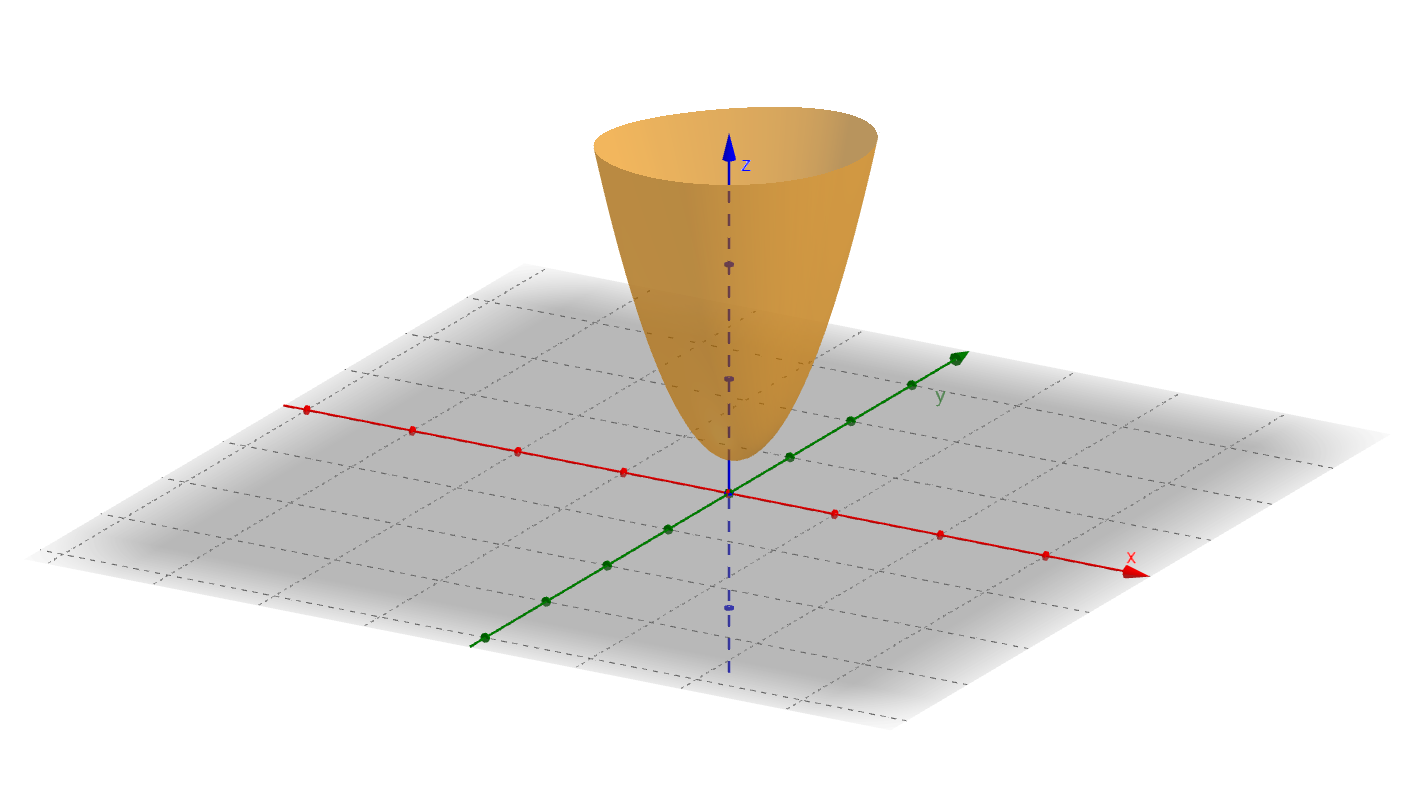
\includegraphics[width=0.75\linewidth]{chapters/chapter 7/graphing step3.png}
\end{figure}

Այժմ $xy$-հարթության ամեն մի $(x,y)$ կետի վրա բարձրանալով/իջնելով այնքան, որքան այդ կետում $f$-ի արժեքն է, կստանանք մի մակերևույթ, որը կլինի $f(x,y)$-ի գրաֆիկը։ Որպես կանոն այն նման է օդում փռված սփռոցի կամ թաշկինակի։ 

Նկատենք, որ ի տարբերություն մեկ փոփոխականի դեպքի՝ այստեղ ունենք
\begin{itemize}
   \item մեկի փոխարեն երկու առանցք
   \item երկու ուղղության փոխարեն\marginnote{հարթության մեջ ձախ/աջ չկա} անվերջ թվով ուղղություններ 
   \item հետևաբար նաև \textit{չկա աճել/նվազելու գաղափար} 
\end{itemize}
Մնացածը, կարելի է ասել, նույնն է, ինչ միաչափ դեպքում։

Լավ է մեկ անգամ տեսնել, քան հարյուր անգամ լսել․ լավ հասկանալու համար պետք է նայել \href{https://www.khanacademy.org/math/multivariable-calculus/thinking-about-multivariable-function/ways-to-represent-multivariable-functions/a/multidimensional-graphs}{տարբեր ֆունկցիաների} գրաֆիկներ։\marginnote{էլ ո՞ւր առանց \href{https://www.desmos.com/3d}{\rm Desmos}-ի ու \href{https://www.geogebra.org/3d}{\rm GeoGebra}-ի} Դե իսկ \href{https://www.intmath.com/vectors/3d-grapher.php}{երկու անգամը՝} պարզապես սքանչելի է։

Նշենք, որ երկուսից ավել փոփոխականների դեպքում գրաֆիկը դժվար է պատկերացնել, դրա համար օգտագործում են տարբեր մեթոդ\-ներ (ասենք՝ երրորդ փոփոխականի արժեքից կախված փոփոխում կետի չափսը կամ գույնը, ավելացնում անիմացիա կամ \href{https://en.wikipedia.org/wiki/Chernoff_face}{ժպիտ}): Մենք կբավարարվենք գծելով $f(x,y)$ տեսքի ֆունկցիայի գրաֆիկներ։


\section{Մասնակի ածանցյալ}

Վերադառնանք նախորդ էջում սահմանած $f(x, y)$
\hyperref[3d_graph]{\color{OliveGreen}ֆունկցիային}, որում $x$-ն ու $y$-ը խնձորի և դեղձի գներն են, իսկ ֆունկցիայի արժեքը՝ մեր եկամուտը։ 

\question{Ինչպե՞ս կչափեք, թե խնձորի արժեքը մի փոքր բարձրացնե\-լիս որքան է փոխվում եկամուտը։}

Կամ որ նույնն է՝ ինչպե՞ս հաշվենք $f(x,y)$-ի փոփոխությունը $x$-ը փոխելիս։ Դեղձի գինը՝ $y$-ը պահենք ֆիքսված, և $x$-ին փոքրիկ աճ տալով՝ շարունակենք ինչպես սովորական ֆունկցիայի ածանցյալի դեպքում․
\[
\lim_{h \to 0} \frac{f(x + h, y) - f(x, y)}{h}
\]
\marginnote{եթե $f$-ը մեկ փոփոխականի է՝ $\dfrac{df}{dx}$\\ եթե մի քանի փոփոխականի է՝ $\dfrac{\partial f}{\partial x}$}Ահա այս թիվը կանվանենք $f$-ի \textit{մասնակի ածանցյալ} ըստ $x$-ի և կնշանակենք $f_x$ կամ $\partial_x f$ կամ էլ՝ $\dfrac{\partial f}{\partial x}$։

\begin{definition}
Եթե հետևյալ սահմանը գոյություն ունի և անվերջ չէ՝
\[
f_x = \lim_{{h \to 0}} \frac{f(x + h, y) - f(x, y)}{h}
\]
ապա այն կանվանենք $f$ ֆունկցիայի \textbf{մասնակի ածանցյալ} ըստ $x$-ի։ Նույն կերպ սահմանում ենք նաև $f$-ի մասնակի ածանցյալն ըստ $y$-ի՝
\[
f_y = \lim_{{h \to 0}} \frac{f(x,y + h) - f(x, y)}{h}
\]
\end{definition}

$f_x$-ը ցույց է տալիս $f$-ի փոփոխման արագությունը միմիայն $x$-ը փոխելիս, այսինքն՝ երբ շարժվում ենք միայն $x$-երի ուղղությամբ, իսկ $y$-ին ձեռք չենք տալիս՝ պահում ենք հաստատուն։ Նույն ձևով, բնականաբար, $f_y$ = $f$-ի արագությունը $y$-ը փոխելիս՝ $x$-ը թողնելով անշարժ։

\begin{example}
Եթե $f(x, y) = x^2 + y^2$, ապա $f_x$-ը հաշվելիս համարում ենք, որ $y$-ը հաստատուն թիվ է՝
\[
f_x= (x^2)' + (y^2)' = 2x + 0 = 2x
\]
իսկ $f_y$-ը հաշվելիս՝ համարում ենք, որ $x$-ն է հաստատուն․
\[
f_y = (x^2)' + (y^2)' = 0 + 2y = 2y
\]
\end{example}

Նկատենք, որ ինչպես սովորական ֆունկցիայի ածանցյալի դեպքում, $f_x(x,y)$-ն ու $f_y(x,y)$-ը $x$-ից և $y$-ից կախված ֆունկցիաներ են և տարբեր կետերում ընդունում են տարբեր արժեքներ։

\begin{example}
Եթե $g(x, y) = 4x^{100}y$, ապա կրկին, նախ կհամարենք $y$-ը հաստատուն.\marginnote{$(\text{հաստատուն} \cdot f)' = \text{հաստատուն} \cdot f'$}
\[
f_x = 400x^{99}y
\]
հետո՝ $x$-ը․
\[
f_y = 4x^{100}
\]
\end{example}

Փաստորեն երկու փոփոխականի դեպքում ունենք ոչ թե մեկ, այլ երկու արագություն։ Եկեք այդ երկու մասնակի արագությունները խմբավորենք և գրենք մեկ վեկտորով՝
\[
\begin{bmatrix}
f_x \\ f_y
\end{bmatrix}
\]

Ստացված վեկտորը կոչվում է $f$ ֆունկցիայի \textbf{գրադիենտ} և նշանակվում է՝ $\nabla f(x,y)$։ Այն երկու ($x$-երի և $y$-ների ուղղությամբ) արագություններից կազմված վեկտորն է, և մասնավորապես վերևի օրինակում՝
\[
\nabla f(x, y) = \begin{bmatrix}
    400x^{99}y \\ 4x^{100}
\end{bmatrix}
\]

\warning{Գրադիենտը տարբեր կետերում ընդունում է տարբեր ար\-ժեքներ․ $\nabla f(\vx)$-ը ոչ թե ֆիքսված վեկտոր է, այլ $\vx=(x,y)$-ից կախված վեկտոր-ֆունկցիա։}

Նկատենք, որ չնայած $f(x,y)$-ի գրաֆիկը գծում ենք $3$ առանցք ունեցող եռաչափ տարածության մեջ, նրա գրադիենտը $2$-չափանի վեկտոր է։ Սովորաբար այն գծում ենք $xy$-հարթության մեջ, և որքան մեծ լինեն մասնակի ածանցյալները, այնքան ավելի երկար վեկտոր կլինի գրադիենտը տվյալ կետում։ 

Նման \marginnote[*+1]{նշանակենք $\vx = \begin{bmatrix}
    x_1 & \dots & x_n
\end{bmatrix}$} ձևով սահմանում ենք նաև ցանկացած $n$ թվով փոփոխականնե\-րից կախված $f(x_1,\dots,x_n)=f(\vx)$ ֆունկցիայի մասնակի ածանցյալները՝
\begin{align*}
f_{x_1}(\vx) &= \frac{\partial f}{\partial x_1}(\vx) = \lim_{{h \to 0}} \frac{f(x_1 + h, x_2, \ldots, x_n) - f(x_1, x_2, \ldots, x_n)}{h}\\
f_{x_2}(\vx) &= \frac{\partial f}{\partial x_2}(\vx) = \lim_{{h \to 0}} \frac{f(x_1, x_2+h, \ldots, x_n) - f(x_1, x_2, \ldots, x_n)}{h} 
\\
&\qquad \qquad \qquad \qquad \qquad  \vdots  \\
f_{x_n}(\vx) &= \frac{\partial f}{\partial x_n}(\vx) = \lim_{{h \to 0}} \frac{f(x_1, x_2, \ldots, x_n + h) - f(x_1, x_2, \ldots, x_n)}{h}
\end{align*}
և նրա գրադիենտը՝
\[
\nabla f(\vx) =
\begin{bmatrix}
f_{x_1}(\vx) &
f_{x_2}(\vx) &
\dots &
f_{x_n}(\vx)
\end{bmatrix}
\]
որը այս դեպքում լինում է $n$-չափանի վեկտոր։

\question{Ենթադրենք $f(\vx)=\va \cdot \vx$, որտեղ $\va$-ն ինչ-որ մի ֆիքսված վեկտոր է։ Ի՞նչ կարծում, ո՞րն է $\nabla f$-ը։}

\section{Շղթայի կանոն}

Մի քանի փոփոխականի ֆունկցիայի մասնակի ածանցյալներն ունեն գրեթե նույն հատկություններն ու կանոնները, ինչ իրենց մեկ փոփոխա\-կա\-նանոց ազգականները։ Մասնավորապես, երբ ածանցում ենք ըստ, ասենք, $i$-րդ փոփոխականի՝ $x_i$-ի,
\begin{align*}
(f \pm g)_{x_i}(\vx) &= f_{x_i}(\vx) \pm g_{x_i}(\vx)\\
(c \cdot f)_{x_i}(\vx) &= c \cdot f_{x_i}(\vx)
\end{align*}
և արտադրյալի դեպքում՝
\[
(f \cdot g)_{x_i}(\vx) = f_{x_i}(\vx)  \cdot  g(\vx) + f(\vx) \cdot g_{x_i}(\vx)
\]

% \item \[\frac{\partial}{\partial x_i} (f(\vx) \pm g(\vx)) = \frac{\partial f(\vx)}{\partial x_i} \pm \frac{\partial g(\vx)}{\partial x_i}\]
        
% \item \[\frac{\partial}{\partial x_i} (c \cdot f(\vx)) = c\cdot\frac{\partial f(\vx)}{\partial x_i} \]

% \item \[\frac{\partial}{\partial x_i} (f(\vx) \cdot g(\vx)) = \frac{\partial f(\vx)}{\partial x_i} \cdot g(\vx) + f(\vx) \cdot \frac{\partial g(\vx)}{\partial x_i}
% \]

\begin{example}
% \marginnote{խոստանում ենք այլևս չգունավորել}
Հաշվենք $f\cdot g$-ի մասնակի ածանցյալները, որտեղ $f(x,y) = {\color{myblue}{2x^2}}$ և $g(x,y) ={\color{myred}{4x + 6y}}$․
\begin{align*}
(f\cdot g)_{x} &= {\color{myblue}{4x}}  \cdot {\color{myred}{(4x + 6y)}} + {\color{myblue}{2x^{2}}} \cdot {\color{myred}{4}} = 24x^{2} + 24xy\\
(f\cdot g)_{y} &= {\color{myblue} 0}\cdot {\color{myred}{(4x + 6y)}} + {\color{myblue}{2x^{2}}} \cdot {\color{myred} 6} = 12x^{2}
\end{align*}
Իհարկե կարող էինք նաև $f\cdot g$-ի մեջ տեղադրել $f$-ի ու $g$-ի բանա\-ձևերը, բազմապատկել, բացել փակագծերը, հետո նոր ածանցել, բայց այսպես ավելի կարճ է և հարմար։
\end{example}

Այնուամենայնիվ, այստեղ կա մի բան, որ չկար մեկ փոփոխականի դեպքում։ Երբ ունենք մեկից ավելի փոփոխականներ, հնարավոր է, որ մի փոփոխականը կախված լինի մյուսից, և դրանցից մեկի փոփոխությունը ազդի նաև մյուսի փոփոխության վրա։

Պատկերացրեք՝ ունեք սուպերմարկետ, որի եկամտի ֆունկցիան է՝
\[
f(x,y) = 20x^{1.3} + 30y^{2.1}
\]
որտեղ $x$-ը ցույց է տալիս, թե քանի «Դուետ» է վաճառվել, իսկ $y$-ը՝ քանի «Գրանդ Քենդի» սառը թեյ։

Բնականաբար, $x$-ն ու $y$-ը օդի $t$ ջերմաստիճանից կախված փոխվում են․ որքան շոգ է, այնքան ավելի շատ են սառը սուրճ կամ թեյ գնում։ Ասենք՝
\[
x(t) = 400+3t, \qquad y(t) = 500+2t
\]

\question{$t$-ն մի քիչ փոփոխելիս որքա՞ն կփոխվի $f(x,y)$-ը։}
Կամ այլ կերպ ասած՝
\begin{itemize}
    \item եթե $f$-ը կախված է $x$-ից ու $y$-ից
    \item իսկ $x$-ը (կամ $y$-ը, կամ երկուսն էլ) կախված են $t$-ից
    \item ապա որքա՞ն կփոխվի $f$-ը $t$-ն փոխելիս
\end{itemize}

Հարցին պատասխանելու տարբերակներից մեկն է $f(x,y)$-ի մեջ $x$-ի ու $y$-ի փոխարեն տեղադրել դրանց արժեքներն՝ արտահայտած $t$-ով, ապա ստացվածը պարզապես ածանցել ըստ $t$-ի․
\[
f(x, y) = 20x^{1.3} + 30y^{2.1}
= 20(400+3t)^{1.3} + 30(500+2t)^{2.1} = f(t)
\]

Այս տարբերակը ձանձրալի է, և մյուս կողմից՝ ցանկալի կլիներ օգտա\-գոր\-ծել $x$-ի ու $y$-ի փոփոխման արագությունները ($t$-ից կախված)։ Փոխարենը կա մի այսպիսի պարզ ու հասարակ կանոն՝\marginnote[*+1]{կամ որ նույնն է՝ \[f_s = f_xx_s + f_yy_s\]}
\[
\frac{\partial f}{\partial t} = \frac{\partial f}{\partial x}\cdot \frac{\partial x}{\partial t} + \frac{\partial f}{\partial y} \cdot \frac{\partial y}{\partial t}
\]
այսինքն՝ որպեսզի պարզենք, թե $t$-ից կախված ի՞նչ արագությամբ է փոփոխվում $f(x,y)$-ը, նայում ենք, թե որքան է նրա արագությունն իր երկու բաղադրիչների՝ $x$-ի և $y$-ի նկատմամբ, ապա ստացված թվերը բազմապատկում դրանցից յուրաքանչյուրի ունեցած արագությամբ ($t$-ի նկատմամբ)։ Նույն կերպ՝ եթե $x$-ն ու $y$-ը կախված լինեին նաև մեկ ուրիշ փոփոխականից, ասենք՝ $s$-ից, կունենայինք՝\marginnote[*+2]{կարծես $\partial x$-երն ու $\partial y$-ները կրճատվեն}
\[
\frac{\partial f}{\partial s} = \frac{\partial f}{\partial x}\cdot \frac{\partial x}{\partial s} + \frac{\partial f}{\partial y} \cdot \frac{\partial y}{\partial s}
\]
Եթե օրինակ $f$-ը կախված լիներ $g$-ից ու $h$-ից, դրանցից յուրաքանչյուրը՝ $x$, $y$, $z$-ից, իսկ վերջիններս էլ՝ $t$-ից ու $s$-ից, ապա $t$-ից կախված $g$-ի փոփոխությունը հաշվելու դեպքում կունենայինք մասնակի ածանցյալների մի այսպիսի շղթա՝
\begin{align*}
f_t &= \text{ (նայում ենք, թե ումի՞ց է կախված $f$-ը) } 
\\
&= f_g g_t + f_h h_t \\
&= \text{ (նույնը $g$-ի և $h$-ի համար) } 
\\ 
&= f_g(g_xx_t + g_yy_t + g_zz_t) + f_h(h_xx_t + h_yy_t + h_zz_t)
\end{align*}
ինչի համար էլ այս բանաձևը հաճախ անվանում են
\textit{շղթայի կանոն։}


\begin{marginfigure}
    \centering
    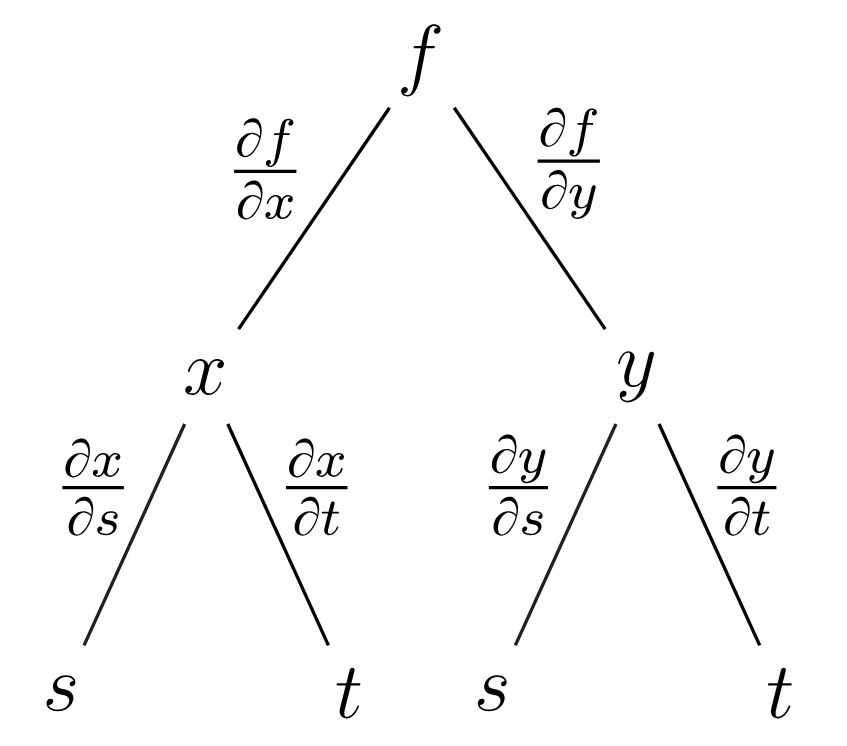
\includegraphics[width=0.75\linewidth]{chapters/chapter 7/chain rule.png}
\end{marginfigure}


\begin{example}
Ենթադրենք $f(x,y)=\sin(x^2+y^2)$, $x=t^2+3$ և
$y=t^3$: Այդ դեպքում՝
\begin{align*}
{f_t}&=f_xx_t+f_yy_t=(2x \cos(x^2+y^2))\cdot (2t)+(2y \cos(x^2+y^2))\cdot(3t^2)\\&=4xt\cos(x^2+y^2)+6yt^2\cos(x^2+y^2)
\end{align*}
Մնում է միայն տեղադրել $x$-ի ու $y$-ի արժեքները։
\end{example}

\begin{example}
Եթե ունենք միայն մեկ փոփոխական՝
\[z(x) = x^2 + 4x\]  
որը կախված է մի ուրիշից՝ \[x(t) = 5t^3 + 2t\]
շղթայի կանոնը դառնում է նույնը, ինչ բարդ ֆունկցիայի ածանցման կանոնը՝ $z(x(t))'=z'(x(t)) \cdot x'(t)$։ Ունենում ենք՝
\begin{align*}
z_t &= z_xx_t= (2x+4)\cdot (15t^2+2)\\&=(2\cdot (5t^3 + 2t)+4)\cdot (15t^2+2)=150 t^5 + 80 t^3 + 60 t^2 + 8 t + 8
\end{align*}
\end{example}

\question{Կարո՞ղ եք ասել այնպիսի ֆունկցիա, որի գրադիենտն է $[2xy \quad x^2+4]$:}


\section{Ուղղությամբ ածանցյալ}

Մի քանի փոփոխական (հետևաբար նաև՝ մի քանի կոորդինատային առանցքներ) ունենալու լավն այն է, որ կարող ենք քայլել լիքը տարբեր ուղղություններով, ոչ թե միայն աջ կամ ձախ։ Մինչդեռ մասնակի ածանցյալները ցույց են տալիս միայն, թե որքան է ֆունկցիայի արա\-գությունը տվյալ կոորդինատային առանցքի երկայնքով շարժվելիս՝ \marginnote{ասենք՝ $f_x$-ը $f$-ի արագությունն է՝ $x$-երի առանցքով աջ ու ձախ շարժվելիս} մնացած բոլոր կոորդինատները թողնելով ֆիքսած։ Իսկ ի՞նչ, եթե ուզում ենք շարժվել ինչ-որ միջանկյալ ուղղությամբ, այսինքն՝ միաժամանակ փոփոխելով մի քանի փոփոխականներ։

Այլ կերպ ասած՝ ի՞նչ կլինի, եթե որոշեք միաժամանակ փոխել և սուրճի, և թեյի գինը, ասենք՝ սուրճը թանկացնեք $h$ դրամով, իսկ թեյը՝ դրանից երկու անգամ ավել, $2h$ դրամով։ Եկամտի ֆունկցիայի արգումենտը այդ դեպքում կդառնա՝
\[
\begin{bmatrix}
    x \\ y
\end{bmatrix}
\mapsto 
\begin{bmatrix}
    x + h \\ y + 2h
\end{bmatrix}
\]
այսինքն՝ կշարժվի $\vv = \begin{bmatrix}
    1 & 2
\end{bmatrix}$ վեկտորի ուղղությամբ ($h$ չափով)։ Ուրեմն ֆունկցիայի/եկամտի փոփոխությունը կկազմի՝
\[
f(\vx+h\vv)-f(\vx)
\]
որը, ինչպես կռահում եք, կբաժանենք փոփոխության չափի՝ $h\|\vv\|$-ի վրա, որպեսզի գտնենք միավոր փոփոխությունը՝
\[
\frac{f(\vx+h\vv)-f(\vx)}{h\|\vv\|}
\]
և վերջապես ի՞նչ եք կարծում, ի՞նչ կանենք, որպեսզի ստանանք $\vv$ ուղղությամբ ֆունկցիայի փոփոխության արագությունը։

\begin{definition}
Ենթադրենք $f(\vx)=f(x_1, \dots, x_n)$ որևէ ֆունկցիա է, իսկ $\vv$-ն՝ որևէ $n$-չափանի վեկտոր։
Եթե հետևյալ սահմանը գոյություն ունի և անվերջ չէ՝\marginnote[*+2]{նշանակում են նաև $D_\vv f$ կամ $\partial_\vv f$}
\[
\nabla_{\vv}{f}(\vx) = \lim_{h \to 0} \frac{f(\vx + h\vv) - f(\vx)}{h\|\vv\|}
\]
ապա այն կանվանենք \textbf{$\vv$-ի ուղղությամբ ածանցյալ} $\vx$ կետում։
\end{definition}

Հարմարության համար սովորաբար կպահանջենք, որ $\vv$ վեկտորի երկարությունը լինի $1$։ Օրինակ $\begin{bmatrix}
    1 & 2
\end{bmatrix}$ վեկտորի փոխարեն կվերցնենք իրեն՝ բաժանած իր երկարության վրա՝ $\begin{bmatrix}
    \dfrac{1}{\sqrt{5}} & \dfrac{2}{\sqrt{5}}
\end{bmatrix}$, և այդ դեպքում $\nabla_\vv f(\vx)$-ի արժեքը չի փոխվի, իսկ հայտարարի $\|\vv\|$-ն կվերանա՝
\[
\nabla_{\vv}{f}(\vx) = \lim_{h \to 0} \frac{f(\vx + h\vv) - f(\vx)}{h} 
\qquad 
\text{(երբ $\|\vv\|=1$)}
\]

\warning{Ի տարբերություն $\nabla f$-ի՝ $\nabla_\vv f$-ը թիվ է, այլ ոչ վեկտոր։ Այն նույնպես տարբեր $\vx$-երում ընդունում է տարբեր արժեքներ։}
\question{Որո՞նք են $[1 \quad 0]$-ի և $[0 \quad 1]$-ի ուղղությամբ ածանցյալները։}


\begin{marginfigure}
    \centering
    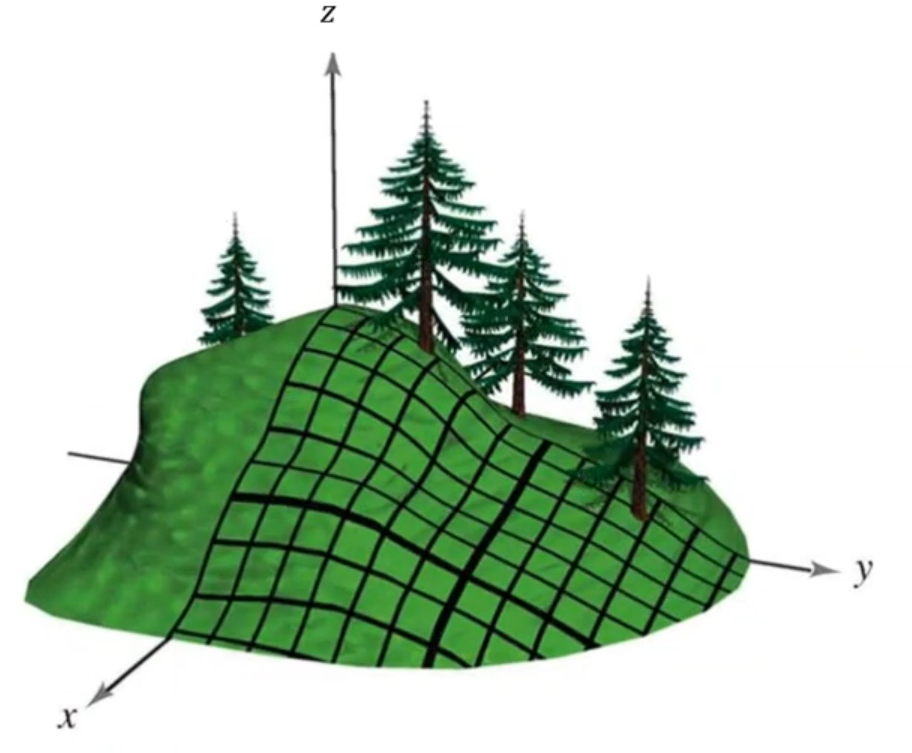
\includegraphics[width=\linewidth]{chapters/chapter 7/forest and peace.png}
\end{marginfigure}

Եթե պատկերացնենք, որ $f(x,y)$-ի գրաֆիկն, ասենք, սարի մակերևույթն է (լանջերը), ապա $xy$-հարթության մեջ գտնվող ցանկացած $\vv$ ուղղու\-թյամբ շարժվելիս սարի լանջով կամ կբարձրանանք, կամ կիջնենք։ $\nabla_\vv f$-ը ցույց է տալիս, թե որքան կկազմի բարձրանալ/իջնելու չափը, եթե մի փոքր քայլ անենք $\vv$ վեկտորի ուղղությամբ։ 

\question{Կարո՞ղ եք գուշակել, թե ինչպես է $\vv=[1 \quad 2]$-ի ուղղությամբ ածանցյալն արտահայտվում ըստ սուրճի ու թեյի գների մասնակի ածանցյալներով։}

Վերոնշյալ $\vv$ վեկտորի ուղղությամբ ածանցելիս, օրինակ, երկրորդ փոփոխականի արժեքը փոփոխում ենք $2$ անգամ ավելի չափով, քան առաջինը, հետևաբար ինչ-որ իմաստով՝ երկրորդի փոփոխման արագությունը պետք է երկու անգամ ավելի մեծ կարևորություն զբաղեցնի, քան առաջինինը։ Պարզվում է, որ իրոք, $\vv$ վեկտորի ուղղությամբ ածանցյալը կարող ենք արտահայտել $\vv$-ի բաղադրիչներով և $f$-ի մասնակի ածանցյալներով հետևյալ կերպ․

\begin{theorem}
Եթե $f$-ը դիֆերենցելի է $\vx$ կետում և $\|\vv\|=1$, ապա
\[
\nabla_\vv f(\vx) = f_{x_1}v_1 + f_{x_2}v_2 + \dots + f_{x_n}v_n
\]
այսինքն՝
\[
\nabla_\vv f(\vx) = \nabla f(\vx_0) \cdot \vv
\]
\end{theorem}

\question{\href{https://www.geogebra.org/m/Bx8nFMNc}{Խաղալով} $P$-ի դիրքի և $\vu$-ի ուղղության հետ՝ կարո՞ղ եք պարզել, թե որ ուղղությամբ է ածանցյալն ամենամեծը։}


\section{Գրադիենտը երկրաչափորեն}

Եթե պատկերացնեք, որ գտնվում եք սարի վրա, որը Ձեր եկամտի ֆունկցիայի գրաֆիկն է (կամ եթե պարզապես ուզում եք բարձրանալ սարի գագաթը), առաջին բանը, որ կուզեք անել՝ Ձեր կանգնած դիրքից շարժվել հնարավորինս վեր։ Այսինքն՝ գրաֆիկասարի յուրաքանչյուր կետում բոլոր հնարավոր ուղղություններից կընտրեք այն ուղղությունը, որով քայլելիս ամենաշատը կբարձրանաք, և կքայլեք այդ ուղղությամբ։ 

Իսկ ինչպե՞ս հասկանանք, թե տվյալ $\vx$ կետում ո՞ր $\vv$ ուղղությամբ գնալիս ենք ամենաշատը բարձրանում, կամ որ նույնն է՝ ո՞ր ուղղությամբ է ֆունկցիայի ածանցյալն ամենամեծը։

\begin{figure}[t]
    \centering
    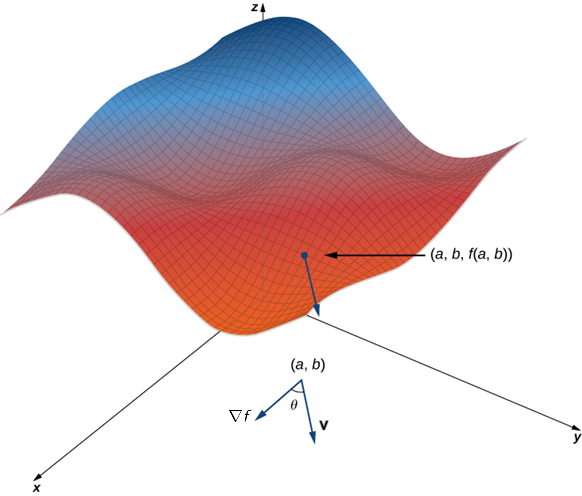
\includegraphics[width=0.75\linewidth]{chapters/chapter 7/grad angle.png}
    \caption*{գտնվում ենք $(a,b)$ կետում}
\end{figure}

Ենթադրենք շարժվում ենք $\vv$ ուղղությամբ և $\|\vv\|=1$: Այդ ուղղությամբ ածանցյալը կլինի՝
\[
\nabla_{\vv}f=\nabla f\cdot \vv
\]
որը, եթե $\nabla f$-ի ու $\vv$-ի կազմած անկյունը նշանակենք $\theta$-ով, կդառնա՝
\[
\|\nabla f\|\cdot \|\vv\| \cdot \cos\theta=  \|\nabla f\|\cos\theta
\]

Բայց $-1 \le \cos\theta \le 1$, հետևաբար $\nabla_\vv f$-ը ամենաշատը կարող է լինել $\|\nabla f\|$, դա էլ միայն այն դեպքում, երբ $\cos\theta$-ն հավասար լինի $1$-ի։ Իսկ 
\[
\cos\theta=1
\quad \text{ նշանակում է } \quad
\theta = 0
\]
և $\vv$-ի ու $\nabla f$-ի ուղղությունները \textit{համընկնում են։} Ստացվեց, որ

\begin{theorem}
\marginnote{ամենադիք վերև ուղղված ուղղությունը} Գրադիենտը ցույց է տալիս ֆունկցիայի \textbf{ամենաարագ աճման ուղղությունը։}
\end{theorem}

Այսինքն եթե գտնվում ենք $(a,b)$ կետում, ապա հաշվելով $\nabla f(a,b)$-ն ու քայլելով ստացված վեկտորի ուղղությամբ՝ կունենանք հնարավոր ամենամեծ աճը։

\question{Իսկ ո՞րն է ֆունկցիայի ամենաարագ \textbf{նվազման} ուղ\-ղու\-թյունը։}

\warning{Հիշենք, որ ածանցյալները ցույց են տալիս ֆունկցիայի աճել/նվազելը միայն տրված կետի մոտիկ շրջակայքում․ $\nabla f$-ի ուղ\-ղությամբ շատ մեծ քայլ անելիս ֆունկցիան կարող է չմեծանալ։}

Սա երկրաչափորեն մեկնաբանում է, թե ինչ վեկտոր է գրադիենտը՝
\begin{itemize}
    \item ուղղությունը $=$ ամենակտրուկ բարձրանալու ուղղությունը
    \item երկարությունը $=$ այդ ուղղությամբ ֆունկցիայի արագությունը
\end{itemize}
և առանցքային դեր է խաղում օպտիմիզացիայի տեսության ու մեքե\-նայական ուսուցման մեջ։


\section{Էքստրեմումի խնդիրը բազմաչափ դեպքում}

Ճիշտ ինչպես \hyperref[single_var_extrema]{\color{OliveGreen}միաչափ դեպքում} ածանցյալի միջոցով որոնում ու գտնում էինք, թե որ կետերում է ֆունկցիան ընդունում իր լոկալ իմաստով ամենամեծ/ամենափոքր արժեքները, նույնը կարող ենք անել նաև այս դեպքում՝ ածանցյալի փոխարեն օգտագործելով դրա բազմաչափ տարբերակը՝ ֆունկցիայի գրադիենտը։

Ենթադրենք ունենք որևէ $f(\vx)=f(x_1,\dots,x_n)$ ֆունկցիա։

\begin{definition}
Կասենք, որ $f(\vx)$-ը $\va$ կետում ընդունում է \textbf{լոկալ մաքսիմում} (մինիմում), եթե $\va$ կետին բավականաչափ մոտ՝\marginnote[*+1.5]{այսինքն՝ $\va$-ից ամենաշատը $\delta$ հեռա\-վորության վրա գտնվող կետերում}
\[
\|\vx-\va\| < \delta
\]
կետերում $f$-ի ամենամեծ (ամենափոքր) արժեքը $f(\va)$-ն է։
\end{definition}

$\va$ կետը համապատասխանաբար կանվանենք ֆունկցիայի \textit{լոկալ մաք\-սի\-մումի (մինիմումի) կետ,} իսկ այդ երկուսը միասին՝ \textit{էքստրե\-մու\-մի կետեր։} Նման ձևով կսահմանենք նաև գլոբալ էքստրեմումի ու կրիտի\-կական կետի գաղափարները։ 


\begin{figure}[b]
\centering %
\floatsetup{floatrowsep=qquad}
\begin{floatrow}[3]%
\ffigbox[\FBwidth]{\caption*{\centering լոկալ մաքսիմում}}{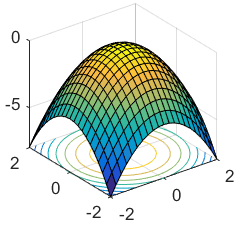
\includegraphics[width=0.4\textwidth]{chapters/chapter 7/local max.png}}
\ffigbox[\FBwidth]{\caption*{\centering լոկալ մինիմում}}{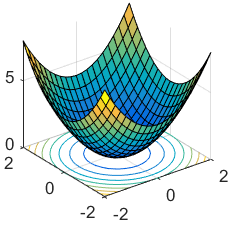
\includegraphics[width=0.4\textwidth]{chapters/chapter 7/local min.png}}
\ffigbox[\FBwidth]{\caption*{\centering թամբի կետ}}{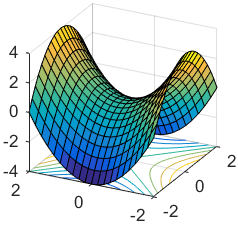
\includegraphics[width=0.4\textwidth]{chapters/chapter 7/saddle point.png}}
\end{floatrow}
\end{figure}


Ինչպես մեկ փոփոխականի ֆունկցիայի դեպքում, այնպես էլ այստեղ․
\begin{theorem}
Եթե $\va$-ն $f$-ի լոկալ կամ գլոբալ էքստրեմումի կետ է և $f$-ը $\va$-ում դիֆերենցելի է, ապա
\[
\nabla f(\va) = \mathbf{0}
\]
\end{theorem}

Եվ նորից, այս պայմանը անհրաժեշտ է, բայց ոչ՝ բավարար․ կրիտի\-կա\-կան կետ լինելը դեռ չի նշանակում, որ կետը էքստրեմումի կետ է։ Այլ կերպ ասած՝ հնարավոր է, որ որևիցե կետում ֆունկցիայի գրադիենտը լինի $\mathbf{0}$, բայց ֆունկցիան չընդունի ոչ լոկալ մաքսիմում, ոչ լոկալ մինիմում։ Այդպիսի կետերը կանվանենք \textit{թամբի կետեր։}

\newpage

\begin{definition}
Կասենք, որ $\va$-ն $f$ ֆունկցիայի\marginnote{անգլերեն՝ {\it saddle point}} \textbf{թամբի կետ} է, եթե այն էքստրեմումի կետ չէ, բայց $\nabla f(\va) = \mathbf{0}$։
\end{definition}

Ինչո՞ւ է կոչվում թամբի կետ։ Որովհետև \href{https://math.libretexts.org/Courses/University_of_California_Davis/UCD_Mat_21C\%3A_Multivariate_Calculus/13\%3A_Partial_Derivatives/13.7\%3A_Extreme_Values_and_Saddle_Points#Second_Derivative_Test_2:~:text=appears\%20in\%20the\%20following\%20figure.}{նման է} թամբի։ Կարող էր կոչվել նաև չիփսի կետ։

\begin{marginfigure}
    \centering
    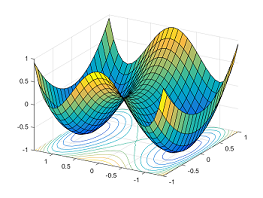
\includegraphics[width=\linewidth]{chapters/chapter 7/many critical points.png}
    \caption*{տիպիկ ֆունկցիա՝ լիքը կրիտիկական կետերով}
\end{marginfigure}

Նման կետերում ֆունկցիայի գրադիենտը զրո է (այսինքն՝ բոլոր մասնակի ածանցյալները $= 0$), սակայն մի փոփոխականը ֆիքսած մյուսը փոփոխելիս՝ ֆունկցիան աճում է, իսկ սա ֆիքսելով՝ առաջինը փոփոխելիս՝ նվազում։ Արդյունքում ստացվում է, որ ֆունկցիան այդ կետում ոչ մեծագույն արժեք է ընդունում, ոչ փոքրագույն։

Որպեսզի պարզենք, թե $f(x,y)$-ի կրիտիկական կետերից որոնք են լոկալ էքստրեմումներ, կօգտվենք նմանատիպ մի արդյունքից, ինչ մեկ փոփոխականի ժամանակ։ Վերցնենք $f$-ի մասնակի ածանցյալները՝ $f_x(x,y)$ և $f_y(x,y)$, ու ածանցենք դրանք ևս մեկ անգամ՝ ըստ յուրաքան\-չյուր փոփոխականի։ Ածանցելով
\begin{itemize}
    \item $f_x$-ը՝ կստանանք $f_{xx} = (f_x)_x$ և $f_{xy} = (f_x)_y$
    \item $f_y$-ը՝ կստանանք $f_{yx} = (f_y)_x$ և $f_{yy} = (f_y)_y$
\end{itemize}
ընդ որում եթե ստացված ածանցյալներն անընդհատ են, ապա ածանց\-ման հերթականությունը կարևոր չէ՝ $f_{xy} = f_{yx}$։

Այժմ հետևյալ մատրիցի՝ \marginnote[*+0.5]{որը կոչվում է $f$-ի \textit{հեսիան}}
\[
    \begin{bmatrix}
        f_{xx} & f_{xy} \\
        f_{yx} & f_{yy}
    \end{bmatrix}
\]
որոշիչը նշանակենք $D$-ով․
\[
D = f_{xx}f_{yy}-f_{xy}^2
\]

Եթե մեկ փոփոխականի դեպքում $f''$-ի նշանը ցույց էր տալիս՝ տրված կրիտիկական կետը էքստրեմումի կետ է, թե ոչ, ապա երկու փոփոխականի դեպքում նույն բանը անում է $D$-ի նշանը։

\begin{theorem}
Եթե $\nabla f(\va) = \mathbf{0}$ ու
\begin{itemize}
    \item $D>0$ և $f_{xx}>0$, ապա $\va$-ն լոկալ մինիմումի կետ է
    \item $D>0$ և $f_{xx}<0$, ապա $\va$-ն լոկալ մաքսիմումի կետ է
    \item $D<0$, ապա $\va$-ն թամբի կետ է
\end{itemize}
\end{theorem}

Նկատենք, որ այս դեպքում ևս $D=0$ կամ $f_{xx}=0$ դեպքերի մասին թեորեմը ոչինչ չի կարող ասել։





\bigskip 

\begin{theory}
.
\begin{itemize}
\item կարդալ [{\rm Stewart}], 880-883 (գրաֆիկ), 900-905 (մասնակի ածանցյալ), 924-925 (շղթայի կանոն), 933-937 (ուղղությամբ ածանցյալ), 946-949 (էքստրեմումներ) էջերը
\item տեսնել մասնակի ածանցյալներն ու գրադիենտը \href{https://youtu.be/GkB4vW16QHI}{սե\-փա\-կան աչքով}
\item ըստ ցանկության՝ դիտել Բ․ Մալթսբիի ներածական \href{https://www.youtube.com/playlist?list=PLBEl4BT8wUgP9lAPqVzuytn09oV_xqTIJ}{տեսա\-դա\-սերը} շատ փոփոխականի ֆունկցիաների մասին 
\item ինչպես նաև Կ․ Քեռյանի խորացված \href{https://www.youtube.com/playlist?list=PLz3NrXxHz_CBamqkX-nPy-hN2iaHmouyo}{դասախոսություններից} 8-րդ և 11-րդ դասերը
\end{itemize}
\end{theory}

\newpage

\section{Խնդիրներ}


\begin{problem}
Հետևյալ ֆունկցիաները համապատասխանեցրեք իրենց գրաֆիկներին․
\begin{enumerate}[label={\alph*}․]
\item $f(x,y) = |x| + |y|$
\item $f(x,y) = |xy|$
\item $f(x,y) = \dfrac{1}{1+x^2+y^2}$
\item $f(x,y) = (x^2-y^2)^2$
\item $f(x,y) = (x-y)^2$
\item $f(x,y) = \sin\left(|x|+|y|\right)$
\end{enumerate}

\begin{figure}[h]
\centering
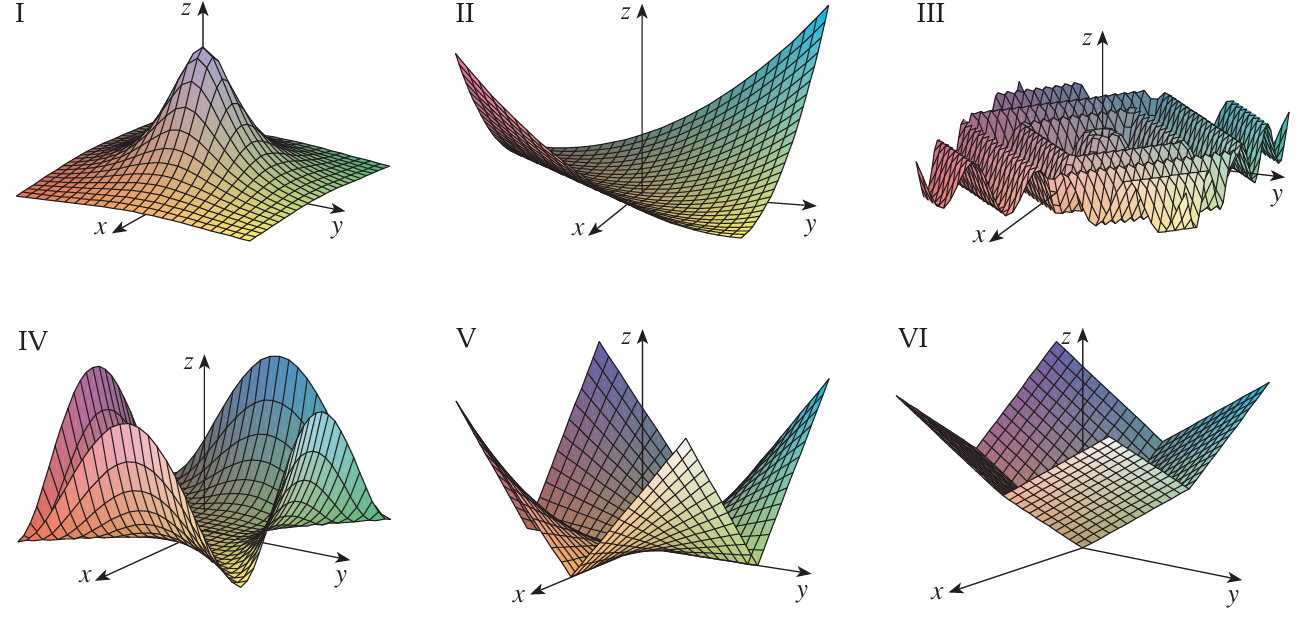
\includegraphics[width=0.75\linewidth]{chapters/chapter 7/match graph.png}
\end{figure}
\end{problem}


\begin{problem}
Գտեք ֆունկցիայի մասնակի ածանցյալները․
\begin{enumerate}[label={\alph*}․]
\item $f(x,y)=3x-2y^2$
\item $f(x,y)=y^7-2x^3+x^2$
\item $f(x,y)=\sin{(xy)}$
\item $f(x,y)=x \cdot \ln y+\dfrac{x}{y}$
\end{enumerate}
\end{problem}


\begin{problem}
Որքա՞ն է $\vv=\begin{bmatrix}
    0.6 & 0.8
\end{bmatrix}$ վեկտորի ուղղությամբ ածանցյալը $(-1,-1)$ կետում․
\begin{enumerate}[label={\alph*}․]
\item $f(x,y) = 3xy$
\item $f(x,y) = 1-x^2$
\item $f(x,y) = e^{x-y}$
\end{enumerate}
\end{problem}


\begin{problem}
Սևանա լճի $(x, y)$ կոորդինատներով կետում ջրի խորությունը 
\[xy^{2}-6x^{2}-3y^{2}\]
մետր է։ $(5, 3)$ կետում գտնվող «Նորատուս» առագաստանավի նավա\-պետը ցանկանում է շարժվել դեպի մի այնպիսի կետ, որում ջուրն ավելի խոր է։ Նրա առաջին օգնականն առաջարկում է նավարկել դեպի հյուսիս, իսկ երկրորդը՝ դեպի հարավ։ Օգնականներից որի՞ խորհուրդը պետք է լսի նավապետը։
\end{problem}


\begin{problem}
Որո՞նք են ֆունկցիայի լոկալ մինիմումի և մաքսիմումի կետերը (եթե կան)․
\begin{enumerate}[label={\alph*}․]
\item $f(x, y) = 3xy$
\item $f(x, y) = x^2-xy$
\item $f(x, y) = 2x^2 - x^3 - y^2$
\item $f(x, y) = x^3 - 3x - y^3 + 3y$
\end{enumerate}
\end{problem}


\begin{problem}
Անհրաժեշտ է $(-5, 0)$, $(1, 7)$, $(9, 0)$ և $(0, -8)$ կոորդինատնե\-րով կետերում գտնվող չորս գյուղերի համար կառուցել հեռուստաաշտարակ։ Ո՞ր $(x, y)$ կետում կառուցենք աշտարակը, որպեսզի գյուղերից դրա ունեցած հեռավորությունների քառակուսիների գումարը լինի հնարա\-վորինս փոքր։
\end{problem}

\hint{Կոորդինատային հարթության մեջ պատկերեք կետերը և գրեք դրանց հեռավորությունը $(x,y)$ կետից։ Ինչի՞ է հավասար դրանց քառակուսիների գումարը։}


\begin{problem}
Ունենք $12$ մ$^2$ մակերեսով ստվարաթուղթ (ինչպես նաև մկրատ ու սոսինձ), որով այս անգամ ցանկանում ենք պատրաստել այսպիսի բաց տուփ (այսինքն առանց վերևի նիստի)՝
\begin{figure}[h]
    \centering
    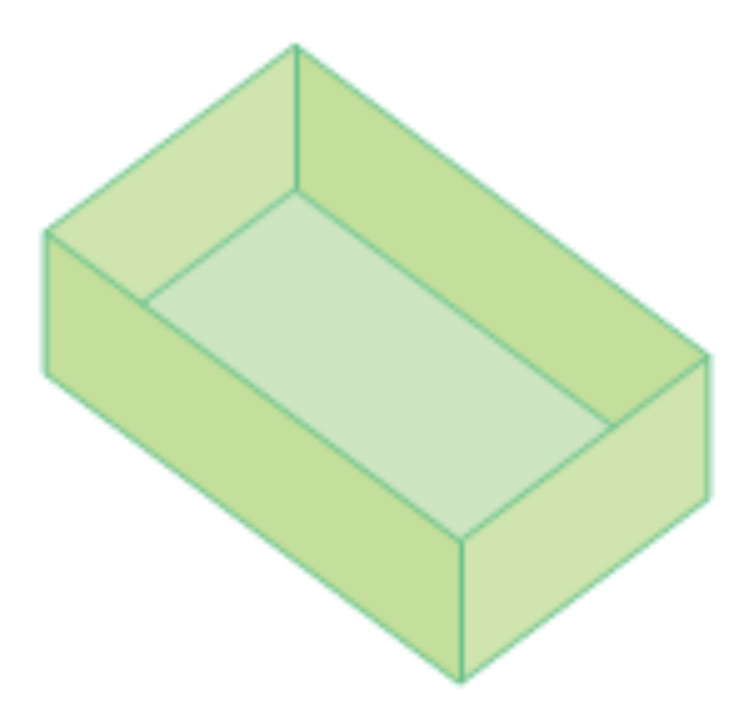
\includegraphics[width=0.4\linewidth]{chapters/chapter 7/topless-box.png}
\end{figure}

Ամենաշատը որքա՞ն կարող է լինել այդ տուփի ծավալը։

\hint{Այս անգամ քառակուսիներ չկան, հետևաբար նշանակենք խորանարդի կողմերը $x$, $y$ և $z$: Կարո՞ղ եք $z$-ն արտահայտել $x$-ով ու $y$-ով։ Իսկ ծավալը՞։}
\end{problem}
